
\chapter{Networks with Nonlinear Autoregressive Dynamics}
\label{chap:five}

The last two chapters combined network models and Hawkes processes to
construct probabilistic models for dynamic neural spike trains. The
key assumption of Hawkes processes, the assumption we leverage to
derive efficient inference algorithms, is that the firing rate is the
sum of non-negative impulse responses from preceding spikes. In other
words, the interactions in a Hawkes process are additive and purely
excitatory. While this leads to interpretable network models for some
systems, in many cases it is more natural to expect a mix of
excitatory and inhibitory interactions. Unfortunately, we cannot have
inhibitory interactions with simple linear dynamics because this could
yield negative firing rates. Instead, we need to revisit the
assumption of linear dynamics.

Chapter~\ref{chap:two} introduced a simple way to generalize the 
linear autoregressive dynamics of the Hawkes process. We retain the 
linear combination of impulse responses from preceding events, but then 
we apply a rectifying nonlinear function to obtain a firing rate. 
Formally, we assume the following model: let,
\begin{align*}
\psi_{t,n} &= \psi_{0,n} + \sum_{n'=1}^N \sum_{d=1}^{D} s_{t-d, n'} \cdot h_{n' \to n}[d], \\
\lambda_{t,n} &= g(\psi_{t,n}), \\
s_{t,n} &\sim p(s_{t,n} \given \lambda_{t,n}, \nu_n)
\end{align*}
where~$\psi_{t,n}$ is a real-valued signal called the
\emph{activation}, ${g: \reals \to \reals_+}$ is a rectifying
nonlinear function that converts the activation into a firing rate,
and the spike count is randomly drawn from a discrete distribution parameterized 
by~$\lambda_{t,n}$ and, potentially, neuron-specific global parameters~$\nu_n$.
Once this nonlinearity has been introduced, the impulse response
functions~$h_{n' \to n}[d]$ are free to be both positive and negative.

This is known as a generalized 
linear model (GLM), and it is widely used in computational neuroscience 
\cite{Paninski-2004, Truccolo-2005, Pillow-2008}. When the spike counts 
are Poisson distributed, then under general conditions~\cite{Paninski-2004} 
the likelihood of the spike counts will be log concave and amenable to 
efficient, exact optimization. Unfortunately, once we introduce nontrivial
prior distributions, like the network models we are considering, 
the posterior becomes multimodal and Bayesian inference becomes more 
challenging. 

This chapter develops efficient MCMC algorithms for approximating the 
posterior distribution of weights in a GLM with prior distributions on the 
impulse responses that are derived from probabilistic network models.
Unfortunately, the augmentation scheme developed for linear Hawkes 
processes is no longer viable due to the nonlinear interactions. Instead,
we develop an inference algorithm based on a recently developed scheme 
known as \polyagamma augmentation. The basic idea behind this scheme is 
to introduce a set of auxiliary variables conditioned upon which the 
discrete spike counts actually ``look'' like Gaussian observations.
Once we have reduced the problem to inference in a linear Gaussian model,
a host of efficient inference algorithms are at our disposal. 


\section{Probabilistic Model}
The underlying model is very similar to the linear autoregressive 
models of the preceding chapter. Rather than considering Poisson 
distributed spike counts, however, here we work with other discrete 
observation models that are amenable to \polyagamma augmentation. 
As we generalize to allow both excitatory and inhibitory interactions, 
we revisit the form of our impulse response and introduce a simpler
form. Finally, we outline a variety of network models that provide 
multivariate Gaussian prior distributions on the interaction weights.

\subsection{Spike count models}

\begin{table}
\begin{center}
\begin{tabular}{c|c|c|c|c}
  \textbf{Name} & Parameters & $p(s \given \psi, \nu)$ & $\bbE[s]$ & $\Var(s)$ \\
  \hline
  Gaussian 
  & $\distNormal(\psi, \nu)$ 
  & $\frac{1}{\sqrt{2 \pi \nu}} e^{ -\frac{1}{2 \nu} (s - \psi)^2}$
  & $\psi$ & $\nu$ \\
  Bernoulli 
  %& $\sigma(\psi)^s \, \sigma(-\psi)^{1-s}$
  & $\distBernoulli(\sigma(\psi))$ 
  & $\frac{(e^\psi)^s}{1+e^\psi}$
  & $\sigma(\psi)$ & $\sigma(\psi) \, \sigma(-\psi)$ \\
  Binomial 
  %& ${\nu \choose s} \, \sigma(\psi)^s \, \sigma(-\psi)^{\nu-s}$
  & $\distBinomial(\nu, \sigma(\psi))$ 
  & ${\nu \choose s} \,\frac{(e^\psi)^s}{(1+e^\psi)^\nu}$
  & $\nu \sigma(\psi)$ & $\nu \sigma(\psi) \, \sigma(-\psi)$ \\
  Neg. Binomial 
  %& ${\nu + s -1 \choose s} \, \sigma(\psi)^s \, \sigma(-\psi)^{\nu}$
  & $\distNegBinomial(\nu, \sigma(\psi))$
  & ${\nu +s - 1 \choose s} \,\frac{(e^\psi)^s}{(1+e^\psi)^{\nu+s}}$
  & $\nu e^\psi$ & $\nu e^\psi / \sigma(-\psi)$ \\
\end{tabular}
\end{center}
\caption{List of observation distributions.}
\label{tab:obs_models}
\end{table}

The spike counts are stochastically drawn from a distribution
parameterized by an underlying, real-valued
\emph{activation},~$\psi_{t,n}$, and a static parameter,~$\nu_n$. 
The \polyagamma augmentation can be applied to observation models 
that depend on a logistic transformation of the activation,
\begin{align*}
  \sigma(\psi) &= \frac{e^\psi}{1+e^\psi},
\end{align*}
which has the property~$\sigma(-\psi) = 1-\sigma(\psi)$. The Bernoulli,
binomial, and negative binomial distributions are all natural choices.
% Since the Poisson distribution can be seen as a limit of either the binomial
% or the negative binomial distribution, we can approximate a Poisson model 
% as well. 
While the Gaussian distribution is not a proper model for discrete
spike counts, we include it in our list since our inference procedure will 
reduce the other models to a Gaussian. Table~\ref{tab:obs_models} 
lists the basic properties of these observation distributions.

The Bernoulli distribution is appropriate for binary spike counts,
whereas the binomial and negative binomial have support
for integer~$s\in \{0, \ldots, \nu\}$ and~$s \in \{0, 1, \ldots \}$, respectively.
Notably missing from this list is the Poisson distribution,
which does not seem to be amenable to the augmentation schemes
we will derive below. Nevertheless, both the binomial and negative
binomial distributions converge to the Poisson under certain
limits, and they afford the added flexibility of modeling under- and
over-dispersed spike counts. Specifically, while the Poisson has unit 
dispersion (its mean is equal to its variance), the binomial distribution 
is always under-dispersed, since its mean always exceeds its variance, 
and the negative binomial is always over-dispersed, with variance greater 
than its mean.

\subsection{Linear Gaussian Activation Model}
As in the previous chapter, we model the impulse response as a weighted 
sum of basis functions,
\begin{align}
\label{eq:glm_impulse}
h_{n' \to n}[d] &= a_{n' \to n} \sum_{b=1}^B w_{n' \to n}^{(b)} \cdot \phi_b[d].
\end{align}
Here, however, we combine the scalar weight and 
the normalized basis function. In this more complicated model, the normalized 
basis function lacks the same simple interpretation of a distribution over 
induced spike times.  Moreover, in some cases, we may even wish to model interactions that 
are both excitatory \emph{and} inhibitory --- for example, the effect of a
spike may be inhibitory at short time scales and excitatory after a certain
delay. While these types of interactions may not correspond to actual biological synapses, they 
can still capture salient autocorrelations in neural spike trains.

Plugging~Eq.~\ref{eq:glm_impulse} into the activation model, we have,
\begin{align}
  \nonumber
  \psi_{t,n} &\triangleq \psi_n^{(0)}  +                 
               \sum_{n'=0}^N  \sum_{b=1}^B a_{n' \to n} \, w_{n' \to n}^{(b)}
               \left( \sum_{d=1}^{D} \phi_{b}[d] \cdot s_{t-d, n'} \right) \\
  \nonumber
             &= \psi_n^{(0)}  + \sum_{n'=0}^N \sum_{b=1}^B a_{n' \to n} \, w_{n' \to n}^{(b)} \, \widehat{s}_{t,n'}^{(b)} \\
  \label{eq:linear_activation}
             &= (\ba_{n} \odot \bw_n)^\trans \, \widehat{\bs}_t,
\end{align}
where~$\psi_n^{(0)}$ is the baseline activation of neuron~$n$,
$\bphi_{b}$ is a basis function 
that weights the previous spike counts for 
offsets~${d \in \{1, \ldots, D\}}$
, the binary variable~${a_{n' \to n} \in \{0,1\}}$ 
indicates whether or not there exists 
a directed connection from neuron~$n'$ to neuron~$n$,
and~$w_{n' \to n}^{(b)}$ captures the influence that
spikes on neuron~$n'$ exert on neuron~$n$ at
offsets weighted by the~$b$-th basis function.  
Since the basis function and the signal 
are assumed to be fixed,  can precompute the inner sum, which is simply the 
convolution of the signal with the basis function, to get~$\widehat{s}_{t,n}^{(b)}$.
Since this is a linear function, we can combine the
connections, weights, and filtered spike trains into
vectors to get the linear form  in Eq.~\ref{eq:linear_activation}.
Here, we have,
\begin{align*}
  \ba_n &=
    \bigg[
      1,  
      & a_{1 \to n}, & & \ldots, & & a_{1 \to n}, 
      & & \ldots, &
      &a_{N \to n}, & & \ldots, & &a_{N \to n} 
    &\bigg]^\trans, \\
  \bw_n &=
    \bigg[
      \psi_n^{(0)}, 
      &w_{1 \to n}^{(1)}, & & \ldots, & &w_{1 \to n}^{(B)}, 
      & &\ldots, &
      &w_{N \to n}^{(1)}, & & \ldots, & &w_{N \to n}^{(B)} 
      &\bigg]^\trans, \\
  \widehat{\bs}_t &=
    \bigg[
      1, 
      &\widehat{s}_{t,1}^{(1)}, & & \ldots, & &\widehat{s}_{t,1}^{(B)}, 
      & &\ldots, &
      &\widehat{s}_{t,N}^{(1)}, & & \ldots, & &\widehat{s}_{t,N}^{(B)} 
    &\bigg]^\trans,
\end{align*}
\sloppy
and~$\odot$ dentoes the elementwise product. Note that each~$a_{n' \to n}$ 
is repeated~$B$ times in the vector~$\ba_{n}$. For convenience, we
let~$\bA$ and~$\bW$ refer to the~${N \times NB+1}$ matrices obtained
by stacking the vectors~$\ba_n^\trans$ and~$\bw_n^\trans$, and we
let~$\widehat{\bS}$ denote the~${T \times NB+1}$ matrix with rows
given by~$\widehat{\bs}_t^\trans$. The major difference between this formulation and that of the standard 
GLM is that here we have explicitly modeled the sparsity of the 
weights via the ``adjacency matrix'' $\bA$. Under the standard 
formulation, all weights are present, that is,~${a_{n' \to n} \equiv 1}$.

Consider a model with one basis function ($B=1$) defined
by,~${\phi_{1,d} = e^{-d/\tau}}$.
Then~$\widehat{s}_{t,n}^{(1)}$ is a weighted sum of spikes in the
window~$[t-D,t-1]$, where the weights decay
according to an exponential function with time constant~$\tau$.  
If~${a_{n' \to n}=1}$, indicating a
connection from neuron~$n'$ to neuron~$n$, and
the weight,~$w_{n' \to n}^{(1)}$, is positive, the influence will be
excitatory. If it is negative, the effect will be inhibitory.
Together, the weights~$\bW$ define a functional \emph{network} of
interactions.

\subsection{Network Models}
With this new impulse response model, each edge of the network 
is now associated with a~$B$-dimensional weight vector. We can 
use the same adjacency matrix models as in the previous chapters,
but we need to consider new models for the weight matrix. A 
multivariate Gaussian prior is a natural choice. We consider 
weight models of the form,
\begin{align*}
  p(\bw_n \given \{\bz_n\}, \bvartheta) 
  &= \distNormal(w_n^{(0)} \given \mu_0, \sigma^2_0 ) \prod_{m=1}^N 
     \distNormal(\bw_{n' \to n} \given \bmu_{n' \to n}, \, \bSigma_{n' \to n}), \\
  &= \distNormal(\bw_n \given \bmu_n, \bSigma_n),
\end{align*}
where~$\bmu_{n' \to n}$ and~$\bSigma_{n' \to n}$ are the mean and covariance,
and they implicitly depend on the latent variables,~$\bz_{n'}$ and~$\bz_n$, and
the parameters of the network model,~$\bvartheta$.
The last line combines the Gaussian factors into single multivariate Gaussian prior
with parameters,
\begin{align}
  \bmu_n 
    &= \begin{bmatrix}
      \mu_0 \\
      \bmu_{1 \to n} \\
      \vdots \\
      \bmu_{N \to n}
    \end{bmatrix}, & \text{ and } & &
  \bSigma_n 
  &= \begin{bmatrix}
    \sigma_0^2 &                     &        & \\
               & \bSigma_{1 \to n}   &        & \\
               &                     & \ddots & \\
               &                     &        & \bSigma_{N \to n} 
    \end{bmatrix}.
\end{align}
As previously mentioned, the parameters~$\rho_{n' \to n}$,~$\bmu_{n' \to n}$, and~$\bSigma_{n' \to n}$ 

\begin{table}
\begin{center}
\begin{tabular}{c|c|c|c}
Name & $\text{dom}(\bz_n)$ & $\bmu_{n' \to n}$ & $\bSigma_{n' \to n}$\\
\hline
Gaussian Model & --- & $\bmu$ & $\bSigma$ \\
Stochastic Block Model & $\{1, \ldots, K\}$ & $\bmu_{z_{n'} \to z_n}$ & $\bSigma_{z_{n'} \to z_n}$ \\
Latent Distance Model (${B=1}$) & $\reals^K $ & $-||\bz_n - \bz_{n'}||_2^2 + \mu_0$ & $\sigma^2$
\end{tabular}
\end{center}
\caption{Gaussian Weight Models}
\label{tab:W_models}
\end{table}

Table~\ref{tab:W_models} defines the three weight models considered in this chapter.  
Each model defines the mean and variance of a multivariate
normal distribution,~$\bw_{n' \to n} \sim \distNormal(\bmu_{n' \to
  n}, \bSigma_{n' \to n})$.  In the Gaussian model, all weights are
independent and identically distributed.  The stochastic block model,
has parameters for each pair of classes, each drawn from a normal
inverse-Wishart prior,~$(\bmu_{k' \to k}, \bSigma_{k' \to k}) \sim
\distNormalInvWishart(\mu_0, \kappa_0, \Sigma_0, \nu_0)$. Finally, we
consider a latent distance model, but only for the case where the
weights are scalar, i.e.~$B=1$. In this case, the distance between
points is inversely proportional to the mean weight.  For higher order
weights, additional assumptions would be required in order to relate
distance to vector weights. In this model, we assume standard normal
priors on the parameters~$\bz_n$ and~$\mu_0$.  The variance is given
an inverse gamma prior,~$\sigma^2 \sim \distInvGamma(\alpha, \beta)$.

Of course, many other models could be added to this list, and in the
discussion we will consider various extensions. An attractive feature
of this approach is that we may indeed draw on an extensive literature
of network models. For the purposes of this paper, we restrict our
attention to these models, based on latent classes and locations,
which are particularly interpretable and easily visualized.


\section{Inference via Gibbs Sampling}
Inference is the process of evaluating the posterior distribution over latent variables given the observed signal, which is related to the joint distribution by Bayes' rule:
\begin{align}
p(\{\nu_n, \ba_n, \bw_n, \bz_n\}_{n=1}^N, \bvartheta \given \bS)  
  &= \frac{p(\bS, \{\nu_n, \ba_n, \bw_n, \bz_n\}_{n=1}^N, \bvartheta) }{p(\bS)}.
\end{align}
It is computationally intractable to compute this posterior exactly and it has no simple closed form solution, so we must instead resort to approximate methods. 
We use Markov chain Monte Carlo (MCMC) methods to collect samples from this posterior distribution.
% With these samples, we can compute unbiased expectations with respect to the posterior distribution.
% For example, we can compute the expected probability that two neurons belong to the same class, the expected weight of a functional connection between two neurons, or the expected predictive likelihood of heldout test data.

\subsection{Collapsed Gibbs Network Updates}
The most challenging aspect of inference is sampling the
posterior distribution over connections,~$\bA$. In the
dense model, where~$a_{n' \to n} \equiv 1$, the posterior
distribution over weights is often log concave, which
makes it easy to find the MAP estimate and characterize
the local uncertainty around the most likely weights.
When the connectivity matrix is sparse, there are instead
many modes corresponding to different patterns of
connectivity. While this makes inference more challenging,
sparse connectivity is an important feature that
contributes to the interpretability of the model.

Fortunately, we can make posterior inference of the
network considerably more efficient by integrating over
possible weights and sampling the binary adjacency
matrix from its marginal distribution. 
First, consider the Gaussian observation model.
Since~$\psi_{t,n}$ is linear in~$\bw_n$, the likelihood
is conjugate with the Gaussian prior, and hence the
posterior is Gaussian as well. We can
compute the posterior distribution in closed form:
\begin{align}
  \nonumber
  p(\bw_n \given \bS, \ba_n, \{\bz_n\}, \bvartheta)
  &\propto
  \distNormal(\bw_n \given \bmu_n, \bSigma_n) \,
  \prod_{t=1}^T \distNormal(s_{t,n} \given (\ba_n \odot \bw_n)^\trans \, \widehat{\bs}_t, \, \nu_n) \\
  \nonumber
  &= \distNormal(\bw_n \given \bmu_n, \bSigma_n) \,
  \distNormal(\bs_n \given (\ba_n \odot \bw_n)^\trans \, \widehat{\bS}, \, \nu_n \bI) \\
  \label{eq:w_conditional}
  &\propto \distNormal(\bw_n \given \widetilde{\bmu}_n, \widetilde{\bSigma}_n),
\end{align}
where
\begin{align*}
  \widetilde{\bSigma}_n &= \left[ \bSigma_n^{-1} +
  \left(\widehat{\bS}^\trans (\nu_n^{-1} \bI) \widehat{\bS} \right) \odot (\ba_n \ba_n^\trans) \right]^{-1}, \\
  \widetilde{\bmu}_n &= \widetilde{\bSigma}_n \left[ \bSigma_n^{-1} \bmu_n +
  \left(\widehat{\bS}^\trans (\nu_n^{-1} \bI)\bs_n \right) \odot \ba_n \right].
\end{align*}

Given this closed-form Gaussian conditional, we can also compute
the conditional distribution over just~$\ba_n$, integrating out
the corresponding weights,~$\bw_n$:
\begin{align}
  \nonumber
  p(\ba_n \given \widehat{\bS}, \brho_n, \{\bz_n\}, \bvartheta)
  &= \int p(\ba_n, \bw_n \given {\bS}, \{\bz_n\}, \bvartheta) \, \mathrm{d} \bw_n \\
  \nonumber
  &\propto p(\ba_n \given \{\bz_n\}, \bvartheta) \, \int p(\bw_n \given {\bS}, \ba_n, \{\bz_n\}, \bvartheta) \, \mathrm{d} \bw_n \\
  \label{eq:a_conditional}
  &= p(\ba_n \given \{\bz_n\}, \bvartheta) \, \frac{\big| \bSigma_n \big|^{-\frac{1}{2}} \exp \Big \{-\frac{1}{2} \bmu_n^\trans \bSigma_n^{-1} \bmu_n \Big \} }
  {\big| \widetilde{\bSigma}_n \big|^{-\frac{1}{2}} \exp \Big \{-\frac{1}{2} \widetilde{\bmu}_n^\trans \widetilde{\bSigma}_n^{-1} \widetilde{\bmu}_n \Big \}}.
\end{align}
Thus, we can efficiently sample from the conditional
distribution of~$\ba_n$ and~$\bw_n$ by first iterating
over each neuron~${n' \in \{1, \ldots, N\}}$ and sampling
a new value of~$a_{n' \to n}$, fixing the values of~$a_{n'' \to n}$
for~$n'' \neq n$ and integrating out the value of~$\bw_n$.
To do so, we simply evaluate the marginal probability in Eq.~\ref{eq:a_conditional}
for both values of~$a_{n' \to n}$ and resample accordingly.
%This is a valid Gibbs step.
Moreover, note that if~$a_{n' \to n}$, the log determinant and the quadratic
form in the numerator of Eq.~\ref{eq:a_conditional} will cancel with the
corresponding term in the denominator. Thus, if~$\bA$ is $d$-sparse (i.e. 
each neuron  has at most~$p$ incoming edges) evaluating
the marginal probability of~$\ba_n$ has complexity an~$O(p^3)$.
Once~$\ba_n$ has been completely
resampled, we can sample a new value of~$\bw_n$ from its multivariate
Gaussian conditional distribution, given by~Eq.~\ref{eq:w_conditional}.

\subsection{\polyagamma augmentation for discrete observations}
When the observations are not Gaussian, the conditional distribution
of~$\bw_n$ cannot be computed in closed form and the collapsed
updates are intractable. To circumvent this problem, we leverage
recently developed augmentation schemes for Gaussian models with
discrete observations \cite{polson2013bayesian, Pillow2012}. The
idea is to augment the observations,~$s_{t,n}$, with auxiliary
variables,~$\omega_{t,n}$, such that conditioned upon the
auxiliary variables, the discrete likelihood appears Gaussian.

First, notice that the discrete likelihoods in Table~\ref{tab:obs_models}
can all be put into  a ``standard'' form in which the probability
mass function can be written,
\begin{align*}
  p(s \given \psi, \nu) &= c(s, \nu) \, \frac{(e^\psi)^{a(s, \nu)}}{(1+e^\psi)^{b(s, \nu)}},
\end{align*}
for some functions,~$a$,~$b$, and~$c$ that do not depend on~$\psi$.
The integral identity at the heart of the P\'{o}lya-gamma augmentation scheme  is
\begin{align}
\label{eq:pg_identity}
\frac{(e^{\psi})^a}{(1+e^{\psi})^b} = 2^{-b} e^{\kappa \psi} \int_{0}^{\infty} e^{-\omega \psi^2 /2} \, p_{\mathrm{PG}}(\omega \given b, 0) \, \mathrm{d}\omega,
\end{align}
where~${\kappa=a-b/2}$ and~$p(\omega\given b, 0)$ is the density of the P\'{o}lya-gamma
distribution~${\distPolyaGamma(b, 0)}$, which does not depend on $\psi$.

Using Eq.~\ref{eq:pg_identity} along with priors~$p(\psi)$ and~$p(\nu)$, we can write the joint density of $(\psi, s, \nu)$ as
\begin{align}
  \label{eq:pg_joint}
  \nonumber
  p(s, \nu, \psi)
  &= p(\nu) \, p(\psi) \, c(s, \nu) \frac{(e^\psi)^{a(s, \nu)}}{(1+e^\psi)^{b(s, \nu)}} \\
  &= \int_0^\infty
  p(\nu) \, p(\psi) \, c(s, \nu) \, 2^{-b(s, \nu)} e^{\kappa(s, \nu) \psi} e^{-\omega \psi^2/2} \, p_{\mathrm{PG}}(\omega \given b(s, \nu), 0) \; \mathrm{d}\omega.
\end{align}
The integrand of Eq.~\ref{eq:pg_joint} defines a joint density on $(s, \nu, \psi, \omega)$ which admits $p(s, \nu, \psi)$ as a marginal density.
Conditioned on these auxiliary variables $\omega$, we have that the likelihood as a function of~$\psi$ is,
\begin{align*}
  p(s \given \psi, \nu, \omega)
  &\propto e^{\kappa(s, \nu) \psi} e^{- \omega \psi^2/2} 
\propto \distNormal \left(\frac{\kappa(s, \nu)}{\omega} \, \bigg| \, \psi, \, \frac{1}{\omega} \right).
\end{align*}

Thus, we effectively have a Gaussian likelihood for~$\psi$, after conditioning 
on~$s$ and~$\omega$. Now we can apply this augmentation scheme to the full
model, introducing auxiliary variables,~$\omega_{t,n}$ for each spike count,~$s_{t,n}$.
Given these variables, the conditional distribution of~$\bw_n$ can be computed in closed form,
as before. Let,
\begin{align*}
  \bkappa_n
  &= \begin{bmatrix} \kappa(s_{1,n}, \nu_n), &\ldots, &\kappa(s_{T,n}, \nu_n)
  \end{bmatrix}^\trans,
\end{align*}
and
\begin{align*}
  \bOmega_n &= \diag \left(
  \begin{bmatrix}
    \omega_{1,n}, & \ldots, & \omega_{T,n}
  \end{bmatrix}
  \right).
\end{align*}
Then we have~$
  p(\bw_n \given \bS, \ba_n, \{\bz_n\}, \bvartheta, \bomega_n, \nu_n)
  \propto \distNormal(\bw_n \given \widetilde{\bmu}_n, \widetilde{\bSigma}_n)$,
where
\begin{align*}
  \widetilde{\bSigma}_n &= \left[ \bSigma_n^{-1} +
  \left(\widehat{\bS}^\trans \bOmega_n \widehat{\bS} \right) \odot (\ba_n \ba_n^\trans) \right]^{-1}, \\
  \widetilde{\bmu}_n &= \widetilde{\bSigma}_n \left[ \bSigma_n^{-1} \bmu_n +
  \left(\widehat{\bS}^\trans \bkappa_n \right) \odot \ba_n \right].
\end{align*}

Having introduced auxiliary variables, we must now also derive
Markov transitions to update them as well. Fortunately, the
\polyagamma distribution is designed such that the conditional
distribution of the auxiliary variables is just a ``tilted'' \polyagamma
distribution,
\begin{align}
  p(\omega_{t,n} \given s_{t,n}, \nu_n, \psi_{t,n})
  &= p_{\mathrm{PG}}(\omega_{t,n} \given b(s_{t,n}, \nu_n), \, \psi_{t,n}).
\end{align}
These auxiliary variables are conditionally independent and hence can
be updated in parallel. Moreover, efficient algorithms are available
to generate \polyagamma random variates~\cite{windle2014sampling}, and
we have ported these to Python\footnote{\url{https://github.com/slinderman/pypolyagamma}}.

\subsection{Observation Parameter Updates}
The observation parameter updates depend on the particular distribution.
For Gaussian observations,~$\nu_n$ is the observation variance, and
it is conjugate with an inverse gamma prior.
Bernoulli observations have no parameters.
In the binomial model,~$\nu_n$ corresponds to the maximum number of
possible spikes --- this is best set a priori.
For negative binomial spike counts, the shape parameter~$\nu_n$ can
be resampled as in~\cite{Zhou2012}.


\subsection{Sampling Network Variables and Parameters}
As before, the latent variables and parameters of the network are relatively 
easy to resample for a given network. The stochastic block model priors are 
conjugate with the Gaussian distributed weights. The locations of the latent 
distance model are not conjugate, but we can update them with hybrid Monte Carlo
\cite{Neal10}.

\subsection{Model Selection}
We have constructed a probabilistic model that supports a variety
of network models, including the four adjacency models and the three
weight models described above. How can we compare these models in
a principled manner? We argue that the typical approach of measuring
predictive log likelihood on held-out time bins is insufficient, since
it relies only on having accurately estimated the network,~$\bA$ and~$\bW$.
It doesn't matter how likely that network is under the latent variable
model, predictive likelihood on held-out time bins only measures the
quality of the network at making predictions. Instead, we advocate
for an alternative measure based on predicting the activity of held-out
neurons. To perform well on this task, we must first learn an accurate
model for the structure underlying the network so that we can
sample latent variables for the new neuron, which in turn allow us to
sample a weighted set of functional connections for that neuron and
finally compute the predictive log likelihood.

The objective we measure is the probability of a new spike
train~$\bs_{n^*}=[s_{1,n^*}, \ldots, s_{T,n^*}]$, given the
observed spike train. To compute this, we must integrate
over the latent variables and parameters underlying the
observed spike train, as well as those underlying the
new spike train. 
Let~$\bV = \{\{\bw_n, \ba_n, \nu_n, \bz_n\}_{n=1}^N, \bvartheta\}$, and
let~$\bv_{n^*} = \{\nu_{n^*}, \bw_{n^*}, \ba_{n^*}, \bz_{n^*}\}$.
This objective can be written,
\begin{align}
  p(\bs_{n^*} \given \bS) &\approx
  \int p(\bs_{n^*} \given \bv_{n^*}, \bS) \, p(\bv_{n^*} \given \bV) \, p(\bV \given \bS) \,
  \mathrm{d} \bv_{n^*} \, \mathrm{d} \bZ \\
  &\approx
  \frac{1}{L} \sum_{\ell=1}^L p(\bs_{n^*} \given \bv_{n^*}^{(\ell)}, \bS),
\end{align}
where
\begin{align}
  \bv_{n^*}^{(\ell)} &\sim p(\bv_{n^*} \given \bV^{(\ell)}),
  &\text{ and }& & 
  \bV^{(\ell)} &\sim p(\bV \given \bS).
\end{align}
The samples~$\{\bV^{(\ell)}\}_{\ell=1}^L$ are the posterior samples generated
by the MCMC algorithm presented above. For each sample, we
sample a new set of latent variables and connections for neuron~$n^*$,
given the parameters included in~$\bV^{(\ell)}$. These, combined with
the spike train, enable us to compute the likelihood of~$\bs_{n^*}$.

This approach constitutes a minor approximation:
the new spike train and the original spike train are not
conditionally independent. It is possible that there are
significant connections from~$n^*$ to neurons in the training
population, and if we had known those connections, we would
have inferred different latent variables and parameters for
the training population. We assume that these effects are small,
i.e. we would find similar class assignments even without observing~$n^*$.
This is reasonable if we are only considering a single neuron~$n^*$
and the training population is relatively large.
In fact, this assumption is fundamental to the generalized
linear model. Without it, the inferred weights and predictions
would be highly sensitive to the addition of a single neuron.
In practice this is rarely the case.


\section{Results}
We demonstrate the efficacy of this approach by applying our framework 
to two neural populations for which we have longstanding experimental 
evidence in favor of a particular latent variable representation.
First, we consider a population of simultaneously recorded retinal 
ganglion cells (RGCs), which can be characterized by their type 
(either \textit{on} or \textit{off} in this dataset) and
by the location of their receptive field centers. 
We then consider a population of hippocampal place cells, which encode 
positions in a two dimensional environment. In both cases, our approach 
recovers these latent representations given only the neural spike trains,
without any knowledge of the stimulus or the true location. Finally, 
we assess the advantages of our Bayesian approach and the scalability 
of our algorithm with synthetic data.

\subsection{Retinal Ganglion Cells}
\label{sec:rgc}

\begin{figure}[t!]
  \centering
  \begin{subfigure}[b]{2.25in}
    \centering
    \caption{}
    \vspace{-.2in}
    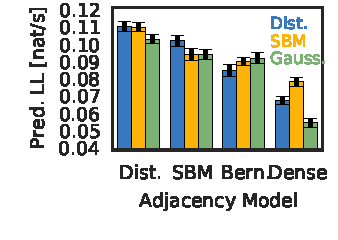
\includegraphics[width=\textwidth]{figures/ch3/rgc_pred_ll_bar.pdf}
    \label{fig:rgc_pll}
  \end{subfigure}
  ~
  \begin{subfigure}[b]{1.6in}
    \centering
    \caption{}
    \vspace{-.2in}
    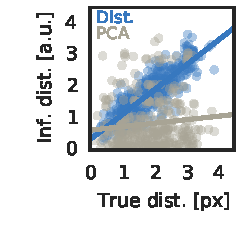
\includegraphics[width=\textwidth]{figures/ch3/rgc_pairwise_distance_scatter.pdf}
    \label{fig:rgc_dist}
  \end{subfigure}
  ~
  \begin{subfigure}[b]{1.6in}
    \centering
    \caption{}
    \vspace{-.2in}
    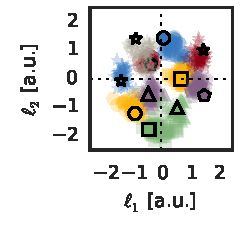
\includegraphics[width=\textwidth]{figures/ch3/rgc_on_locations.pdf}
    \label{fig:rgc_locs}
  \end{subfigure}
  \\
  \vspace{-.2in}
  \begin{subfigure}[b]{1.85in}
    \centering
    \caption{}
    \vspace{-.2in}
    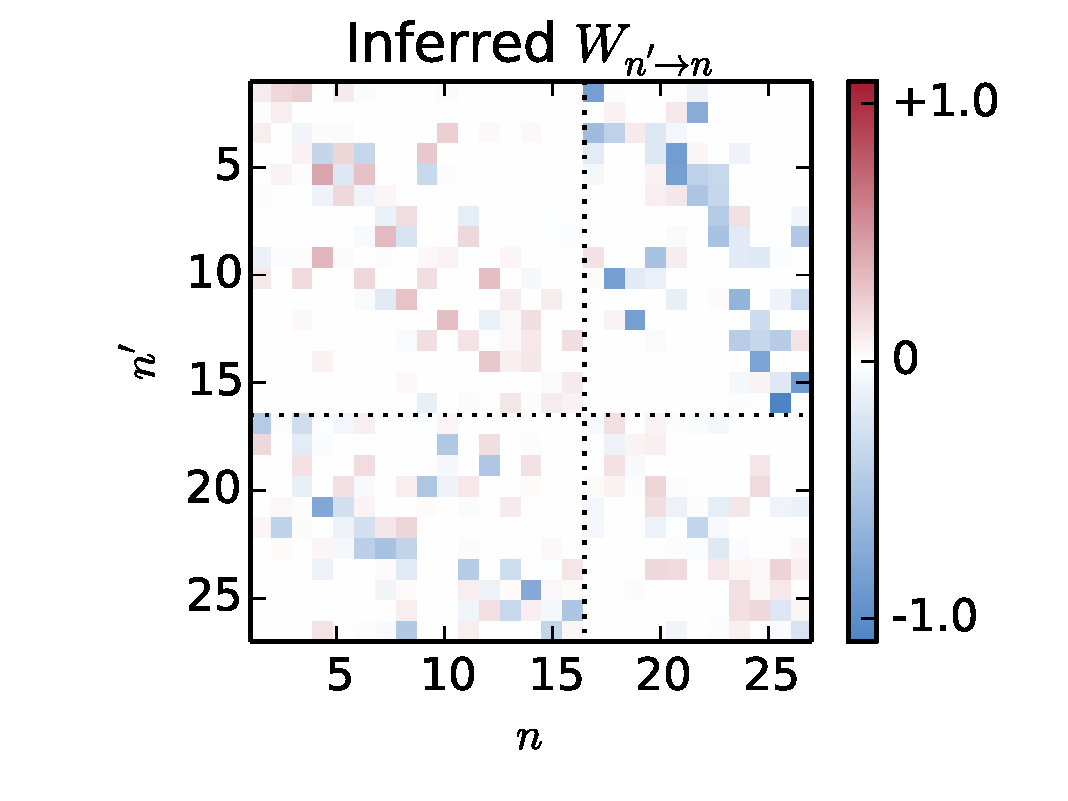
\includegraphics[width=\textwidth]{figures/ch3/rgc_connectivity.pdf}
    \label{fig:rgc_w}
  \end{subfigure}
  ~
    \begin{subfigure}[b]{1.85in}
    \centering
    \caption{}
    \vspace{-.2in}
    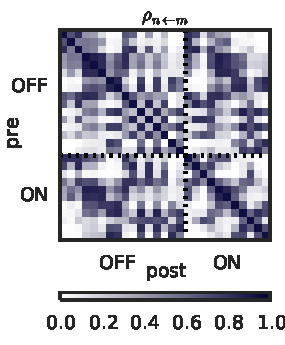
\includegraphics[width=\textwidth]{figures/ch3/rgc_prob_conn.pdf}
    \label{fig:rgc_rho}
  \end{subfigure}
  ~
  \begin{subfigure}[b]{1.85in}
    \centering
    \caption{}
    \vspace{-.2in}
    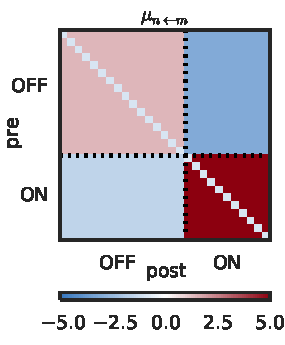
\includegraphics[width=\textwidth]{figures/ch3/rgc_mean_conn.pdf}
    \label{fig:rgc_mu}
  \end{subfigure}
  \vspace{-2em}
  \caption[Retinal ganglion cell types and locations inferred
    from spike trains alone]
          {Retinal ganglion cell types and locations can be inferred
    from spike trains alone.
    \textbf{(a)} The combined distance model and block model yields the highest predictive log likelihood (units: nats/spike), compared to other combinations of adjacency models (groups of bars) and weight models (\textit{blue}: latent distance weight model, \textit{yellow}: stochastic block model for weights, \textit{green}: Gaussian weights).
    \textbf{(b)} The inferred distances under the latent distance model are highly correlated with the true distances, as measured by stimulus sensitivity, whereas inferred embeddings under PCA are not.
    \textbf{(c)} Moreover, the inferred locations (semitransparent markers) recover the true receptive field centers (solid markers with black outline). Shown here only for ON cells.
    \textbf{(d)} Inferred network,~${\bA \odot \bW}$, under a latent distance model of connection probability and a stochastic block model for connection weight, averaged over 500 posterior samples.
    \textbf{(e)} Expected probability of connection under the latent distance model.
    \textbf{(f)} Expected connection strength under the stochastic block model. The inferred cell classes perfectly match the true ON and OFF types, and reflect within-class excitation and between-class inhibition.
}
  \label{fig:rgc}
\end{figure}

We applied our model to simultaneously recorded multineuronal spike
trains from a population of 27 primate retinal ganglion cells
(RGCs). This dataset was previously analyzed with a standard
generalized linear model in \cite{Pillow-2008}.  In this dataset, the
population is presented with a Gaussian white noise video with pixel
sizes tuned to approximately the width of a receptive field. We
trained our models on one minute of spiking activity, binned at one
millisecond time resolution. There were approximately 50,000 spikes in
this recording.  We also held out one minute of data for model
evaluation.

Retinal ganglion cells respond to light (or the absence thereof) shown
upon their receptive field. The cells are roughly evenly distributed
across the two-dimensional retinal plane. Thus, it is natural to
characterize these cells by the location of their receptive field
center.  Moreover, this population is comprised of two types of cells,
\textit{on} and \textit{off} cells, characterized by their response to
visual stimuli. \textit{On} cells increase their firing when light is
shone upon their receptive field; \textit{off} cells decrease their
firing rate in response to light in their receptive field.  Cell types
are identified by similarity in their response properties as well as
morphological and physiological properties~\cite{sanes2015types}. With
knowledge of the stimulus, these cells can be clearly separated into
their respective types by clustering the spike-triggered average
simulus.  This characterization in terms of latent locations and cell
types has been validated through decades of experiments, and has been
made possible by the relative ease with which relevant stimuli can be
identified and controlled. To what extent can these latent
representations be discovered from the spike trains alone?

\sloppy
We fit our model to the measured spike trains for each of the twelve
probabilistic network priors shown above --- three weight models and
four adjacency models. Predictive likelihood comparisons on the
held-out data reveal that the adjacency matrix, i.e. the pattern of
connectivity, is well-characterized by a two-dimensional latent
distance model (Fig.~\ref{fig:rgc_locs}), as expected given the
localized receptive fields of RGCs. Moreover, the pairwise distances
between the latent locations are highly correlated with the true
distances between receptive field centers (Fig.~\ref{fig:rgc_dist}),
even though the stimulus was never used during training. By contrast,
the inferred locations given by the top two principal components of
the spike trains are highly uncorrelated, indicating that PCA does not
recover a meaningful spatial embedding.  Finally, the inferred
locations can be rotated and scaled such that they match the true
locations almost perfectly (Fig.~\ref{fig:rgc_locs}). Rotation does
not change the pairwise distances and scaling simply changes the
units. This matching is highly unlikely for randomly distributed
locations.  In Fig.~\ref{fig:rgc_locs}, the true locations are shown
as solid markers with black outlines, and the inferred locations
sampled from the posterior distribution are shown as semitransparent
markers of the same color and shape.

For the weight matrix, a latent distance model (Dist) and a stochastic
block model (SBM) both yield similar predictive likelihoods. Looking
into the inferred types under the SBM, we find that the neurons are
grouped according to their true \textit{on} and \textit{off} cells,
again without any knowledge of the stimulus. These types determine 
the expected interaction weight for each pair of neurons. 

Figure~\ref{fig:rgc_w} shows the inferred functional network under the
latent distance adjacency model and stochastic block model for
weights.  The neurons are sorted first by their type (\textit{off}
then \textit{on}) and then by their $x$-location. This yields the
three bands in the matrix of connection
probabilities~\ref{fig:rgc_rho}. Nearby cells have much higher
probability of connection. The mean connection strength
(Fig.~\ref{fig:rgc_mu}) shows the characteristic pattern of positive
weights between cells of the same type and negative weights betewen
cells of opposite types. The diagonal of this matrix shows the weights
of self-connections, which are typically negative due to refractory
effects. 

Together, these inferred types and locations provide 
compelling evidence for a highly structured pattern of functional 
connectivity. Given the extensive work on characterizing retinal 
ganglion cell responses, we have considerable evidence that the 
representation we learn from spike trains alone is indeed the 
optimal way to characterize this population of cells. This 
lends us confidence that we may trust the representations learned from 
spike trains recorded from deeper brain areas, where traditional 
stimulus-response correlations are less valuable.

\subsection{Hippocampal Place Cells}
\label{sec:hipp}

\begin{figure}[t!]
  \centering
  \vspace{-.2in}
  \begin{subfigure}[b]{1.75in}
    \centering
    \caption{}
    \vspace{-.2in}
    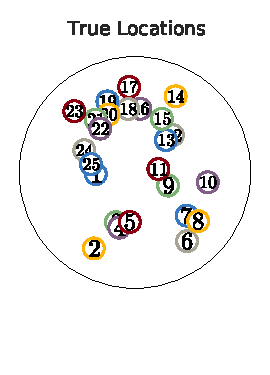
\includegraphics[width=\textwidth]{figures/ch3/hipp_true_locations.pdf}
    \label{fig:hipp_true_locs}
  \end{subfigure}
  ~
  \begin{subfigure}[b]{1.75in}
    \centering
    \caption{}
    \vspace{-.2in}
    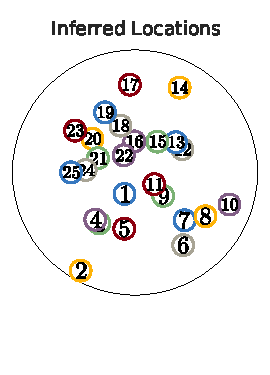
\includegraphics[width=\textwidth]{figures/ch3/hipp_inferred_locations.pdf}
    \label{fig:hipp_inf_locs}
  \end{subfigure}
  ~
  %\begin{subfigure}[b]{1.75in}
  %  \centering
  %  \caption{}
  %  \vspace{-.2in}
  %  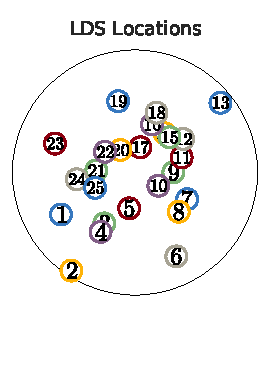
\includegraphics[width=\textwidth]{figures/ch3/hipp_lds_locations.pdf}
  %  \label{fig:hipp_lds_locs}
  %\end{subfigure}
  %\\
  %\vspace{-.2in}
  \begin{subfigure}[b]{1.75in}
    \centering
    \caption{}
    \vspace{-.2in}
    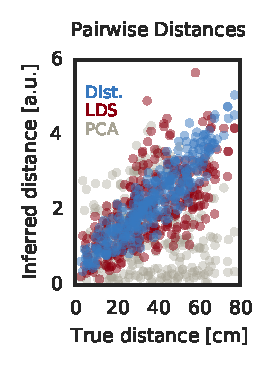
\includegraphics[width=\textwidth]{figures/ch3/hipp_pairwise_distance_scatter.pdf}
    \label{fig:hipp_distances}
  \end{subfigure}
  %~
  \\
  \vspace{-.2in}
  \begin{subfigure}[b]{2.25in}
    \centering
    \caption{}
    \vspace{-.2in}
    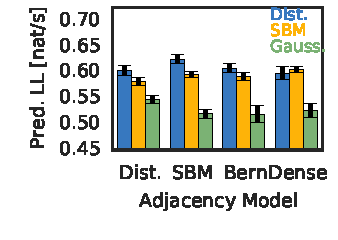
\includegraphics[width=\textwidth]{figures/ch3/hipp_pred_ll_bar.pdf}
    \label{fig:hipp_pll}
  \end{subfigure}
  ~
  \begin{subfigure}[b]{1.85in}
    \centering
    \caption{}
    \vspace{-.2in}
    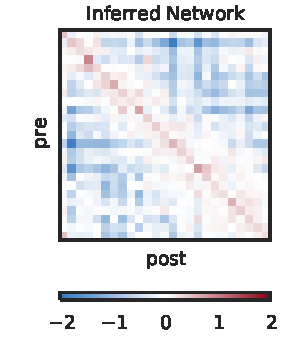
\includegraphics[width=\textwidth]{figures/ch3/hipp_connectivity.pdf}
    \label{fig:hipp_conn}
  \end{subfigure}
  \vspace{-2em}
  \caption[Hippocampal place fields inferred from spike trains]{
    Hippocampal place fields are inferred from population spike trains.
    }
  \label{fig:hipp}
\end{figure}

We also applied our framework to simultaneously recorded
multi-neuronal spike trains from the hippocampus of freely moving rats
in a circular arena.
% Experiments were conducted under the supervision of the
% Massachusetts Institute of Technology (MIT) Committee on Animal Care
% and followed the NIH guidelines.  The micro-drive arrays containing
% multiple tetrodes were implanted above the right dorsal hippocampus
% of male Long-Evans rats.  The tetrodes were slowly lowered into the
% brain reaching the cell layer of CA1 two to four weeks following the
% date of surgery.  Recorded spikes were manually clustered and
% sorted.
This dataset consists of~$N=25$ neurons recorded for a duration of
almost ten minutes and binned in 250ms time bins.  The rat is freely
foraging in an open field environment roughly 120cm in diameter.
% Since place cells are primarily active during location, the spike
% train is segmented into individual running epochs by discarding bins
% in which the velocity is less than 10cm/s.  This results in a
% dataset that is approximately 2000 time bins in length.

As in the retina, we have strong intuitions about the latent structure
underlying hippocampal place cell activity, namely, we expect cells
representing nearby locations to be correlated and cells with disjoint
place fields to be anticorrelated. Can we extract the spatial layout
of place fields from spike trains alone?

We apply our framework, fitting all twelve network models and
evaluating them on the basis of predictive likelihood. We use a
negative binomial observation model to allow multiple spikes per time
bin. We find that the distance dependent weight models yield the
highest predictive likelihood (Fig.~\ref{fig:hipp_pll}). The
stochastic block model yields the highest predictive likelihood, but
upon futher investigation we find that almost all neurons are
connected in this model. There is one outlier, neuron \#$1$, which is
only sparsely connected. The SBM assigns 24 neurons are assigned to
one cluster, and assigns neuron \#$1$ to its own group.  Thus, the
stochastic block model is quite similar to an independent Bernoulli
model, as is evident from the similar predictive likelihood of these
two models.

Looking into the inferred locations under the latent distance model
for the weight matrix, we find that the inferred locations
(Fig~\ref{fig:hipp_inf_locs}) are (up to rotation and scale) highly
similar to the true place field centers (Fig~\ref{fig:hipp_true_locs})
measured using the rat's true location. This is quantified by plotting
the pairwise distances between inferred locations against the pairwise
distances between place field centers. The latent distance model's
pairwise distances are highly correlated with the ground truth,
whereas distances between PCA embeddings are very uncorrelated
(Fig.~\ref{fig:hipp_distances}). For further comparison, we fit a
Poisson linear dynamical system (PLDS) \cite{macke2011empirical} with
a two dimensional latent state space, and used the rows of the
~$N \times 2$ emission matrix as the locations of the neurons. This
sophisticated model, which captures temporal dynamics of the neural
population, yields pairwise distances that are quite correlated with
the true distances, but we find that the variance of this fit grows
with the true distance.  This reflects the fact that the PLDS does not
explicitly parameterize interaction as a function of distance, but
rather induces correlation due to similarity in the emission matrix as
well as shared dynamics.

Finally, we investigated the expected network under the posterior and 
found that upon sorting the neurons by their inferred locations, an
intuitive banded structure emerges (Fig.~\ref{fig:hipp_conn}). 
The positive diagonal indicates strong autocorrelation between a 
neurons spiking in consecutive 250ms bins. Over these time scales, 
self-refractory effects are not evident. The primary connections 
are inhibitory in nature, such that active cells suppress the activity 
of cells with distal place fields. 

These inferred representations again confirm our intuitive beliefs 
about the structure of hippocamapl place cell responses. The 
inferred latent variables recover meaningful structure in the
neural activity, without any access to the location. Instead, 
these representations arise from the neural activity alone.

\subsection{Synthetic Data}
\label{sec:synthetic}

To assess the robustness and scalability of our framework, we apply
our methods to simulated data with known ground truth.  First, we show
that our Bayesian approach can recover structure in larger populations
of neurons than those studied above.  Moreover, we show that our
approach outperforms alternative methods that separate the problems of
finding the network and discovering the underlying structure. Then, we
show that for sparse networks, our approach only scales quadratically
with the number of neurons --- a significant improvement over na\"ive
methods that incur an additional~$O(N^3)$ cost per potential connection.


\subsubsection{Advantages of being Bayesian}
\label{sec:advantages}
\begin{figure}[t!]
  \centering
  \vspace{-.2in}
  \begin{subfigure}[b]{1.8in}
    \centering
    \caption{}
    \vspace{-.25in}
    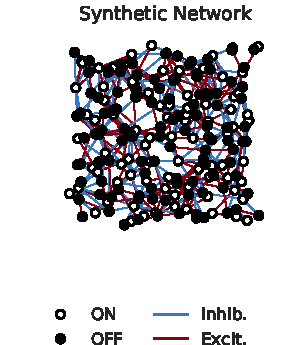
\includegraphics[width=\textwidth]{figures/ch3/synth_rgc_true_network.pdf}
    \label{fig:synth_rgc_true_network}
  \end{subfigure}
  ~
  \begin{subfigure}[b]{1.8in}
    \centering
    \caption{}
    \vspace{-.25in}
    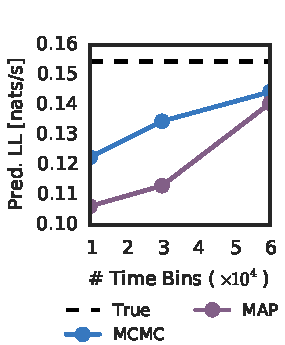
\includegraphics[width=\textwidth]{figures/ch3/synth_rgc_pred_ll.pdf}
    \label{fig:synth_rgc_predll}
  \end{subfigure}
  ~
  \begin{subfigure}[b]{1.8in}
    \centering
    \caption{}
    \vspace{-.25in}
    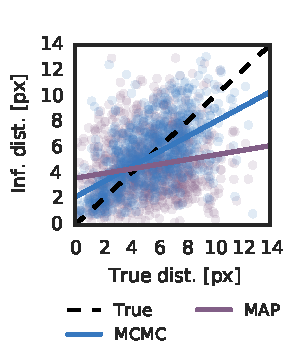
\includegraphics[width=\textwidth]{figures/ch3/synth_rgc_pairwise_distance_scatter.pdf}
    \label{fig:synth_rgc_pairwise_dists}
  \end{subfigure}
  \caption[Synthetic RGC results]{Synthetic results based on the
    retinal ganglion cell population studied above.
    \textbf{(a)} Locations of the 200 neurons (100 \textit{on} and 100 \textit{off} cells) along with a subset of the connections. For clarity, 15\% of the connections are randomly chosen. Though the network is not symmetric, arrowheads are dropped for clarity.
    \textbf{(b)} Predictive likelihood on 10,000 held-out time bins as a function of the number of time bins in the training dataset. ``MCMC'' denotes our Bayesian approach with a latent distance adjacency model and a SBM weight model. ``MAP'' denotes the $L_1$-regularized standard GLM.
    \textbf{(c)} Inferred locations found by our model (MCMC) and by fitting a latent distance model to the thresholded standard GLM network (MAP).
  }
  \label{fig:synth_rgc}
\end{figure}


For these analyses, we simulate a population of 200 neurons with
structure that mimics that of the retinal ganglion cell population
analyzed in Section~\ref{sec:rgc}. Figure~\ref{fig:synth_rgc_true_network}
illustrates the underlying network. As before, we have \textit{on}
cells and \textit{off} cells, each centered at a location in the 2D
retinal plane. Nearby cells are more likely to be functionally
connected, and cells of the same type will have excitatory influence
on one another while cells of different types will inhibit one
another. Again, these functional connections reflect correlations and
anticorrelations between cells that arise from common input. We
simulate 60,000 time bins and tune the network parameters such that if
each time bin were one millisecond, the firing rates would range from 10Hz to
70Hz with a mean of about 30Hz.  Rather than simulating an
external white noise stimulus, here we simulate spontaneous activity
of the network.

Since we know the generative model that gave rise to the data, we can
quantify the improvement from using our fully Bayesian approach
rather than a standard GLM, and compare these improvements to the
upper bound provided by the true model. Figure~\ref{fig:synth_rgc_predll}
shows the predictive log likelihood for 10,000 bins of held-out data as
a function of the number of time bins of training data. For shorter
training datasets, our Bayesian approach yields considerably higher
predictive likelihood than the standard,~$L_1$-regularized GLM. As
the length of the training data increases, both our method and
the standard GLM improve, and ultimately approach the likelihood of
thet true model that generated the data. With more data, the network
inference is driven less by the prior and more by the observations.
Thus, in the limit of infinite data,the GLM will converge to the same
network, and hence the same predictive likelihood, as our Bayesian method.
However, with hundreds of neurons and tens of thousands of time bins,
these results suggest that the Bayesian approach can yield substantial
benefits.

Rather than simultaneously fitting the network and the underlying
latent variables, one may instead fit the network with an
$L_1$-regularized GLM and \textit{then} fit a probabilistic network
model to the GLM connection weights. This is the approach taken
by~\citet{stevenson2009bayesian}.  The advantage is that the network
is only fit once, and since this is usually the most expensive aspect
of inference, it can save considerable time. However, when the data is
limited, both the network and the latent variables are uncertain.  Our
Bayesian approach finds joint assignments with high posterior
probability, whereas the standard GLM finds a single network that does
not account for prior beliefs about structure underlying the network.
In this example, subsequently fitting a latent distance model to the
adjacency matrix of a thresholded GLM network finds an embedding that
is considerably worse than the embedding found by our Bayesian
approach. This is illustrated by the decreased correlation between
true and inferred pairwise distances under the standard GLM compared
to that of our joint, Bayesian approach, as shown in
Figure~\ref{fig:synth_rgc_pairwise_dists}.

\begin{figure}[t!]
  \centering
  \vspace{-.2in}
  \begin{subfigure}[b]{1.8in}
    \centering
    \caption{}
    \vspace{-.25in}
    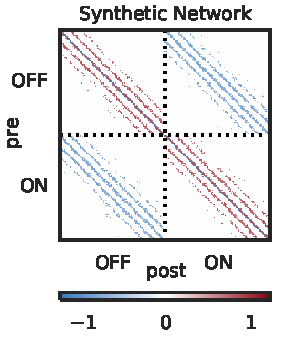
\includegraphics[width=\textwidth]{figures/ch3/synth_rgc_true_conn.pdf}
    \label{fig:synth_rgc_true_conn}
  \end{subfigure}
  ~
  \begin{subfigure}[b]{1.8in}
    \centering
    \caption{}
    \vspace{-.25in}
    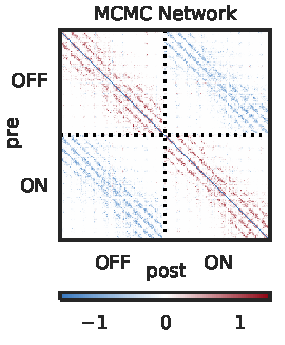
\includegraphics[width=\textwidth]{figures/ch3/synth_rgc_mcmc_conn.pdf}
    \label{fig:synth_rgc_mcmc_conn}
  \end{subfigure}
  ~
  \begin{subfigure}[b]{1.8in}
    \centering
    \caption{}
    \vspace{-.25in}
    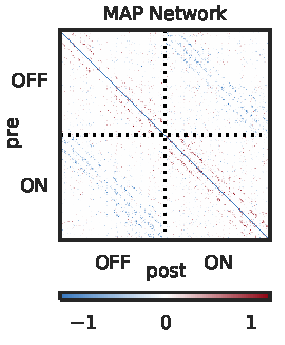
\includegraphics[width=\textwidth]{figures/ch3/synth_rgc_bfgs_conn.pdf}
    \label{fig:synth_rgc_bfgs_conn}
  \end{subfigure} \\
  \begin{subfigure}[b]{1.8in}
    \centering
    \caption{}
    \vspace{-.25in}
    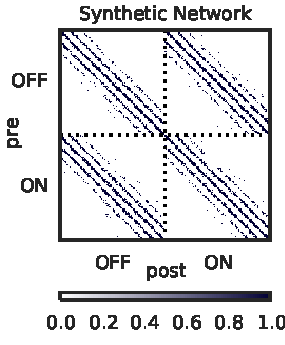
\includegraphics[width=\textwidth]{figures/ch3/synth_rgc_true_sparsity.pdf}
    \label{fig:synth_rgc_true_sparsity}
  \end{subfigure}
  ~
  \begin{subfigure}[b]{1.8in}
    \centering
    \caption{}
    \vspace{-.25in}
    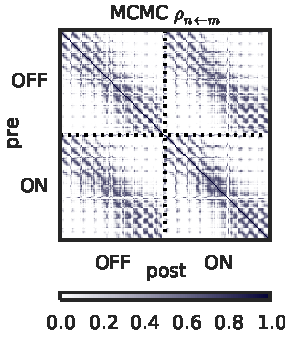
\includegraphics[width=\textwidth]{figures/ch3/synth_rgc_mcmc_prob_conn.pdf}
    \label{fig:synth_rgc_mcmc_prob_conn}
  \end{subfigure}
  ~
  \begin{subfigure}[b]{1.8in}
    \centering
    \caption{}
    \vspace{-.25in}
    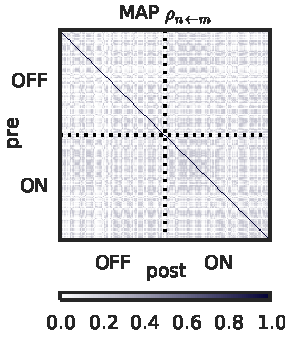
\includegraphics[width=\textwidth]{figures/ch3/synth_rgc_bfgs_prob_conn.pdf}
    \label{fig:synth_rgc_bfgs_prob_conn}
  \end{subfigure}
  \caption[Inferred connection probabilities for synthetic RGC data]{
    \textbf{(a)} Weighted adjacency matrix for the synthetic RGC network shown in Fig.~\ref{fig:synth_rgc_true_network}.
    \textbf{(b)} Network inferred by our fully Bayesian approach.
    \textbf{(c)} Thresholded network found by an~$L_1$-regularized GLM.
    \textbf{(d)} Adjacency matrix corresponding to the true network in Fig.~\ref{fig:synth_rgc_true_conn}.
    \textbf{(e)} Inferred connection probability found by our model with a latent distance prior. The diagonal bands reflect the increased probability for nearby neurons..
    \textbf{(f)} Inferred connection probability found by fitting a latent distance model to the network in Fig.~\ref{fig:synth_rgc_bfgs_conn}. Noise in this network leads to poor location estimates and nearly uniform connection probabilities.
  }
  \label{fig:synth_rgc_prob_conn}
\end{figure}

Figure~\ref{fig:synth_rgc_prob_conn} further illustrates this
point. Here, the true network is shown as a weighted adjacency matrix
(Fig.~\ref{fig:synth_rgc_true_conn}), along with its binary adjacency
matrix (Fig.~\ref{fig:synth_rgc_true_sparsity}). The inferred network
and connection probabilities from our fully Bayesian method with a
latent distance model prior are shown in
Fig.~\ref{fig:synth_rgc_mcmc_conn} and
Fig.~\ref{fig:synth_rgc_mcmc_prob_conn}, respectively. Our MCMC
algorithm does a good job recovering the underlying locations, which
give rise to the diagonally banded connection probabilities, which reflect 
distance dependence.  By
contrast, the MAP network found via an $L_1$-regularized standard GLM
is considerably noisier (Fig.~\ref{fig:synth_rgc_bfgs_conn}), since it
knows nothing of the underlying distance dependent connectivity. A
latent distance model fit to a thresholded copy of this network fails
to capture the distance dependence
(Fig.~\ref{fig:synth_rgc_bfgs_prob_conn}), since the spurious
connections force otherwise well-separated neurons to lie close in the
embedding. By jointly fitting the network and the latent locations, we
weed out these spurious connections.

\subsubsection{Scalability Analysis}

Finally, we address the scalability of our Bayesian inference algorithms.
With large-scale recordings becoming the norm, efficiency is paramount.
There are three major parameters that govern the complexity of inference:
the number of time bins,~$T$; the number of neurons,~$N$; and the level
of sparsity,~$\rho$. The natural unit of measure is the wall-clock time
required to perform one iteration of our MCMC algorithm. The following
experiments were run on a quad-core Intel i5 with 6GB of RAM. Since the
core operations consist of parallelized sampling code and standard linear
algebra, performance scales almost linearly in the number of cores. We
break down the wall-clock time into time spent updating the auxiliary
variables of the observation model and time spent updating the network.
Resampling the latent variables is a negligible cost.

The wall clock time scales linearly with~$T$, as shown in
Figure~\ref{fig:runtime_vs_T}. As we will show in
Section~\ref{sec:methods}, the observation model contains~${NT}$
auxiliary variables, each of which must be resampled. Additionally,
each neuron must compute its sufficient statistics, which involves a
rectangular matrix multiplication costing~$O(TN^2)$ time.

Since there are~$O(N^2)$ possible connections in a network of~$N$
neurons, there is no way to circumvent at least a quadratic cost
in~$N$ (unless some connections can be ruled out \textit{a priori}).
Figure~\ref{fig:runtime_vs_N} shows that this quadratic penalty is
indeed evident. The cost of updating the auxiliary variables is only
linear in~$N$, but the cost of updating the network is quadratic. In
Section~\ref{sec:discussion}, we discuss potential strategies for
ruling out connections and limiting this cost.


\begin{figure}[t!]
  \centering
  \vspace{-.2in}
  \begin{subfigure}[b]{1.81in}
    \centering
    \caption{}
    \vspace{-.25in}
    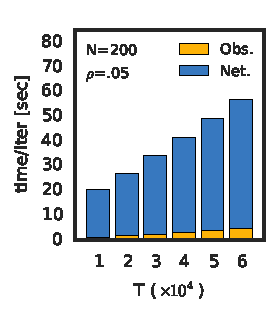
\includegraphics[width=\textwidth]{figures/ch3/runtime_vs_T.pdf}
    \label{fig:runtime_vs_T}
  \end{subfigure}
  ~
  \begin{subfigure}[b]{2.17in}
    \centering
    \caption{}
    \vspace{-.25in}
    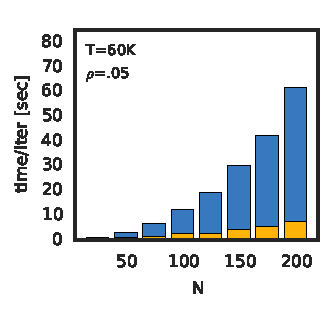
\includegraphics[width=\textwidth]{figures/ch3/runtime_vs_N.pdf}
    \label{fig:runtime_vs_N}
  \end{subfigure}
  ~
  \begin{subfigure}[b]{1.27in}
    \centering
    \caption{}
    \vspace{-.25in}
    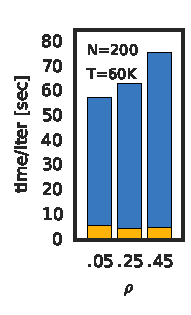
\includegraphics[width=\textwidth]{figures/ch3/runtime_vs_rho.pdf}
    \label{fig:runtime_vs_rho}
  \end{subfigure}
  \vspace{-2em}
  \caption[Scalability of the proposed Bayesian inference algorithm]{
    Scalability of our inference algorithm as a function of: 
    \textbf{(a)} the number of time bins,~$T$;
    \textbf{(b)} the number of neurons,~$N$; and
    \textbf{(c)} the average sparsity of the network,~$\rho$.
    The complexity grows linear with~$T$ and quadratically with~$N$
    (for fixed~$\rho$). The cost is broken down into the cost of
    resampling the \polyagamma auxiliary variables (``Obs.'') and
    the cost of resampling the sparse network (``Net.''). Color
    scheme shared across all panels.
  }
  \label{fig:scalability}
\end{figure}


The total cost could actually be worse than quadratic because the cost
of updating each connection could depend on~$N$. Fortunately, the
complexity of our collapsed Gibbs sampling algorithm only depends on
the number of incident connections received by each neuron,~$p$.
Specifically, we must invert a~$p \times p$ matrix, which incurs
an~$O(p^3)$ cost. Figure~\ref{fig:runtime_vs_rho} illustrates this for
a Bernoulli network with~$N=200$ neurons. The expected number of
incoming connections is related to the probability of connection
by~$\bbE[p]=\rho N$. If we increased the number of neurons but kept
the average in-degree constant, the total cost would scale only
quadratically with~$N$.



\section{Discussion}
\label{sec:discussion}
We have shown that the functional networks underlying
spike trains may provide unique insight into the low-dimensional
structure of neural populations. Looking forward, there are 
two main concerns that we would like to address.
First, ideally we would like algorithms that scale better 
than quadratically with the number of neurons. Second, we 
would like to automate the process of relating the latent 
structure to simultaneously measured environmental cues, stimuli, 
and behavioral correlates. 

\subsection{Further scalability improvements}
For large populations, the bulk of the running time is spent 
sampling the network variables,~$\bA$ and~$\bW$. As the number of
neurons grows, this complexity scales as~$O(N^2)$. To
what extent can we minimize this complexity? As we have shown,
na\"ively applying clustering algorithms and PCA directly
to spike trains does not necessarily yield meaningful features. These
results can be somewhat improved by smoothing the spike
trains (e.g. by taking a moving average), but they are still
fundamentally limited when the low-dimensional structure
lies in the pattern of functional connectivity.

Moreover, our results in Section~\ref{sec:advantages} show that 
separating the problem of inferring the network and discovering 
its latent structure may yield to inferior results. This is 
particularly common for large neural populations, where there is 
substantial posterior uncertainty. 
In practice, we initialize our method with a standard GLM and
find that a small number of iterations of our MCMC algorithm
can yield large improvements in the predictive likelihood of our
model. These improvements come from pruning connections that are
weakly supported by the data, but which are very unlikely under the
prior. This improvement in predictive likelihood is consistent with
existing literature on Bayesian spike-and-slab modeling \cite{Mohamed-2012}.

\sloppy
An alternative approach is to consider models that explicitly limit 
the dimensionality of the network. For example, if we know the 
physical location of neurons (or their approximate location from 
electrode number), we may rule out long-range connections. 
Alternatively, we may constrain the weighted adjacency matrix to be 
low rank, that is ${\bW \odot \bA \equiv \bU \bV^\trans}$, where~$\bU$
and~$\bV$ are rank~${K < N}$. The effect is similar to that of 
a linear dynamical system model~\cite{paninski2010new, macke2011empirical}. 
Unfortunately, it is less clear how to incorporate interpretable 
structure into this type of model, although see~\citet{buesing2014clustered}
for some initial steps in this direction.


Finally, we have developed a Markov chain Monte Carlo inference algorithm,
and while we have shown reasonable performance on recordings of 
hundreds of neurons over tens of thousands of time bins, as we scale 
to larger recordings alternative algorithms may be preferable. 
When the complexity is dominated by the number of time bins, 
stochastic variational inference (SVI)~\cite{Hoffman13} provides 
an attractive alternative. Since the time bins are conditionally 
independent given the network, we can get unbiased estimates of 
sufficient statistics from \textit{mini-batches} of time bins
and use them to inform stochastic mean field updates. 
While we have not derived this mean field algorithm here, it is 
relatively straightforward to derive these algorithms for 
\polyagamma augmented models~\cite{Pillow2012, Zhou2012}. 
Still, the limiting factor will often be the number of neurons, 
in which case SVI is not immediately applicable. Developing 
approximate inference algorithms that only consider subsets of neurons is 
an active area of research~\cite{soudry2015efficient}. 

\subsection{Relating circuit structure to stimuli and behavior}
\TODO{Can we automate the task of relating the inferred latent structure to
simultaneously recorded, but potentially high-dimensional, measurements of 
the environment or the animal's behavior?}
